\subsection{La chaîne d'outils}
\label{sec:toolchain}
Maintenant que nous avons vu les différents outils de la théorie du contrôle que nous avons implémentés pour CHIPS, nous allons voir comment nous avons mis en place la chaîne d'outils permettant d'à partir d'un programme CHIPS, de générer un programme BIP, qui sera ensuite compilé et exécuté pour obtenir les résultats de simulation. \\

\subsubsection{Le fonctionnement de la chaîne d'outils}
\label{sec:explication_toolchain}

La chaîne d'outils fonctionne de la manière suivante : à partir d'un programme CHIPS, le parseur développé lors de la partie \ref{sec:parseur} va générer un AST. Celui-ci sera ensuite utilisé par le programme qui va le sérialiser en un fichier XMI. Ce fichier sera ensuite analysé par un programme python pour vérifier sa validité par rapport au méta-modèle. Si le fichier est valide, il sera ensuite utilisé avec ATL pour générer un fichier XMI, qui lui sera valide par rapport au méta-modèle BIP. Enfin, ce dernier fichier XMI sera utilisé par le compilateur BIP pour générer un programme BIP exécutable. Pour l'instant ce programme ne contient que les composants ainsi que les connecteurs, mais pour l'instant il n'y a pas la logique interne des composants. \\

Une fois le programme BIP généré, on peut écrire la logique interne des composants en BIP, puis générer du code C++ grâce au compilateur BIP. Ce code C++ peut ensuite être compilé et exécuté pour obtenir les résultats de simulation. \\

\subsubsection{Les résultats de la chaîne d'outils}
\label{sec:resultat_toolchain}

Pour illustrer le fonctionnement de la chaîne d'outils, nous avons réutilisé l'exemple du drone que nous avons utilisé dans la partie \ref{sec:anti_windup}. Nous avons donc écrit un programme CHIPS pour le drone, puis nous avons utilisé la chaîne d'outils pour générer un programme BIP, puis du code C++ et enfin exécuter le programme pour obtenir les résultats de simulation. \\

Nous avons trois programmes BIP différents\footnote{Etant donné qu'il n'y a pas la logique interne des composants en BIP les programme CHIPS se ressemble dû à leurs composantes et leurs connections}, un sans anti-windup, un avec l'anti-windup clamp et un avec l'anti-windup back-calculation. Nous avons ensuite exécuté les trois programmes pour obtenir les résultats de simulation. Les résultats sont présentés dans les figures \ref{without_anti_windup_chips_altitude}, \ref{without_anti_windup_chips_integral}, \ref{without_anti_windup_chips_blade}, \ref{clamp_anti_windup_chips_altitude}, \ref{clamp_anti_windup_chips_integral}, \ref{clamp_anti_windup_chips_blade}, \ref{back_calculation_anti_windup_chips_altitude}, \ref{back_calculation_anti_windup_chips_integral} et \ref{back_calculation_anti_windup_chips_blade}. \\

Nous pouvons remarquer quelque chose de flagrant, c'est que les résultats obtenus avec la chaîne d'outils ne sont pas les mêmes que ceux obtenus lorsqu'on qu'on exécutait un programme C++ directement. Cette différence s'explique par le fait que la logique interne du composant PID en BIP utilise des fonctions C++ qui utilisent toutes en type pour ses variables des float, alors qu'en BIP, les variables sont de type double. Cette différence de précision peut donc expliquer les différences de résultats. \\

Il faut quand même noter que même si les résultats ne sont pas les mêmes, ils suivent la même tendance et permettent de comparer les différents anti-windups entre eux. On peut donc conclure que la chaîne d'outils fonctionne correctement et permet de générer un programme BIP à partir d'un programme CHIPS. \\

\begin{figure}
    \centering
    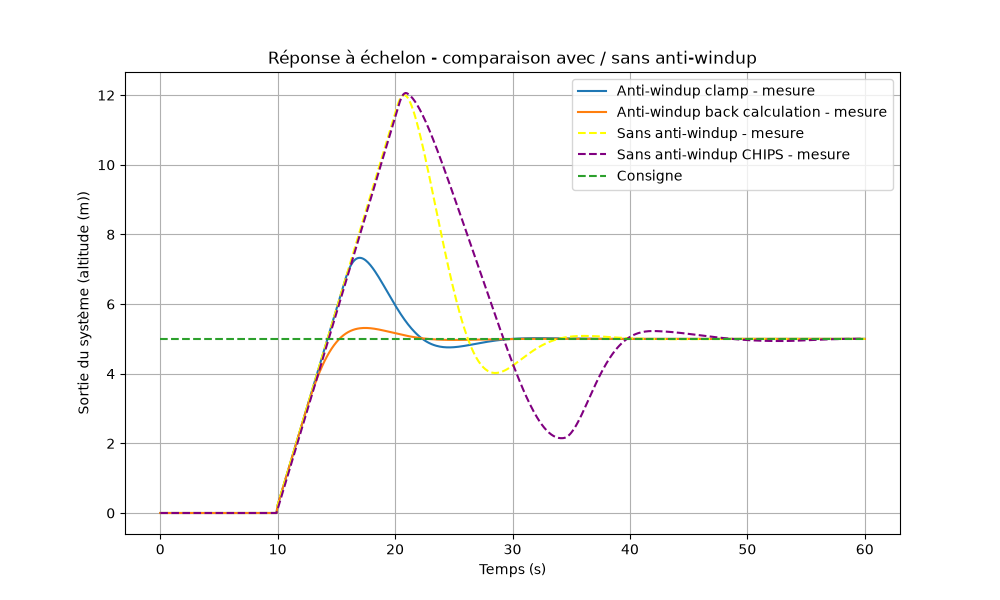
\includegraphics[width=\textwidth]{images/without_anti_windup_chips_altitude.png}
    \caption{Les différentes altitudes du drone avec différents anti-windups comparés à sans anti-windup en CHIPS}
    \label{without_anti_windup_chips_altitude}
\end{figure}

\begin{figure}
    \centering
    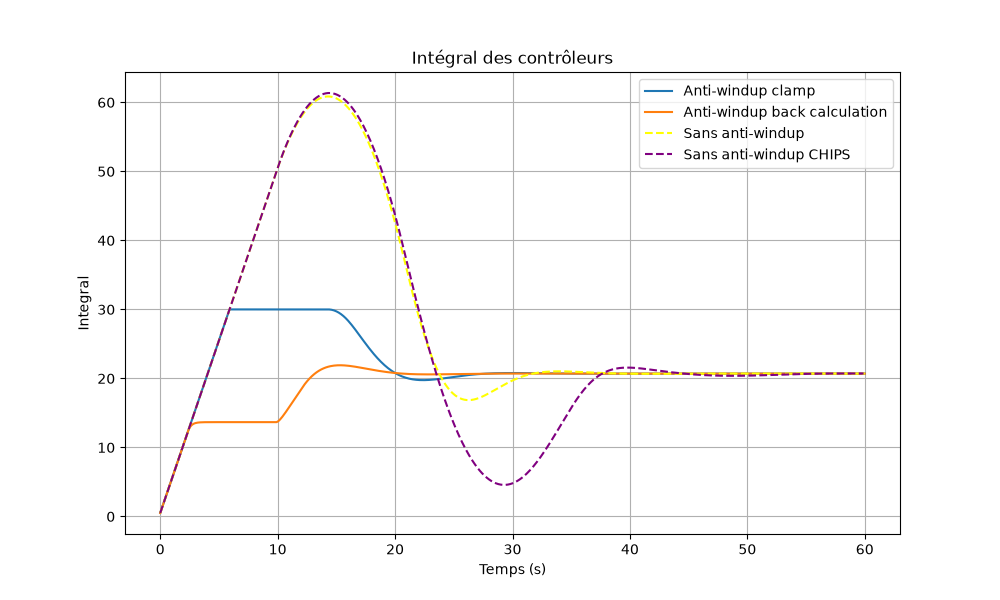
\includegraphics[width=\textwidth]{images/without_anti_windup_chips_integral.png}
    \caption{Les différentes intégrales des anti-windups comparées à sans anti-windup en CHIPS}
    \label{without_anti_windup_chips_integral}
\end{figure}

\begin{figure}
    \centering
    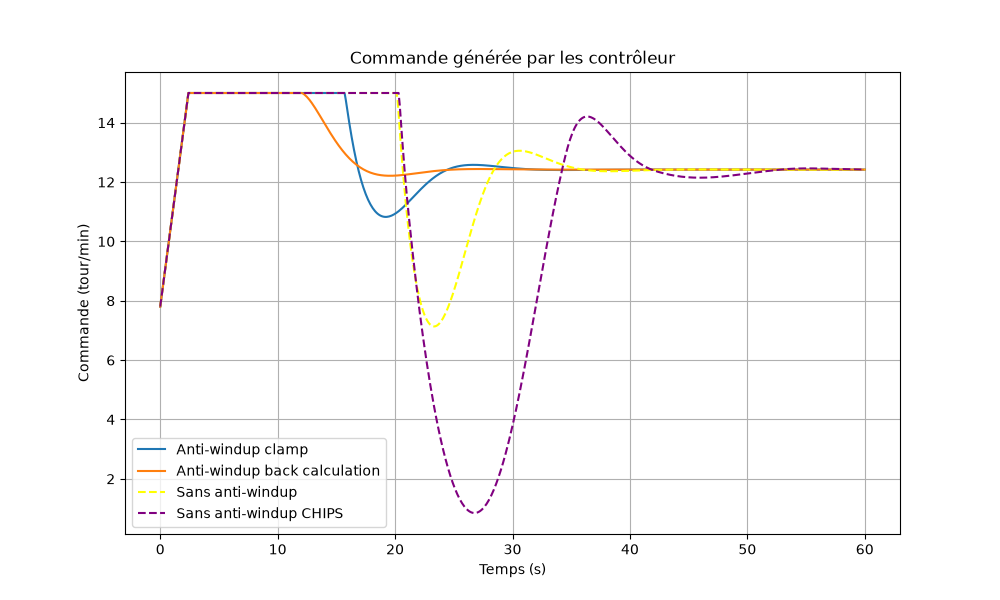
\includegraphics[width=\textwidth]{images/without_anti_windup_chips_blade.png}
    \caption{Les différentes vitesses de rotation des hélices avec différents anti-windups comparées à sans anti-windup en CHIPS}
    \label{without_anti_windup_chips_blade}
\end{figure}

\begin{figure}
    \centering
    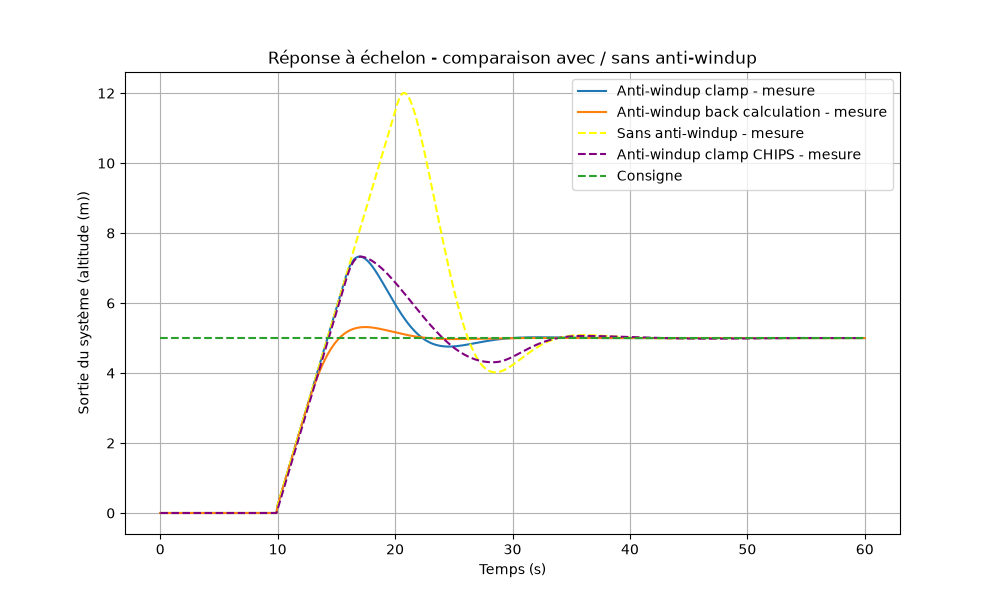
\includegraphics[width=\textwidth]{images/clamp_anti_windup_chips_altitude.png}
    \caption{Les différentes altitudes du drone avec différents anti-windups comparés à l'anti-windup clamp en CHIPS}
    \label{clamp_anti_windup_chips_altitude}
\end{figure}

\begin{figure}
    \centering
    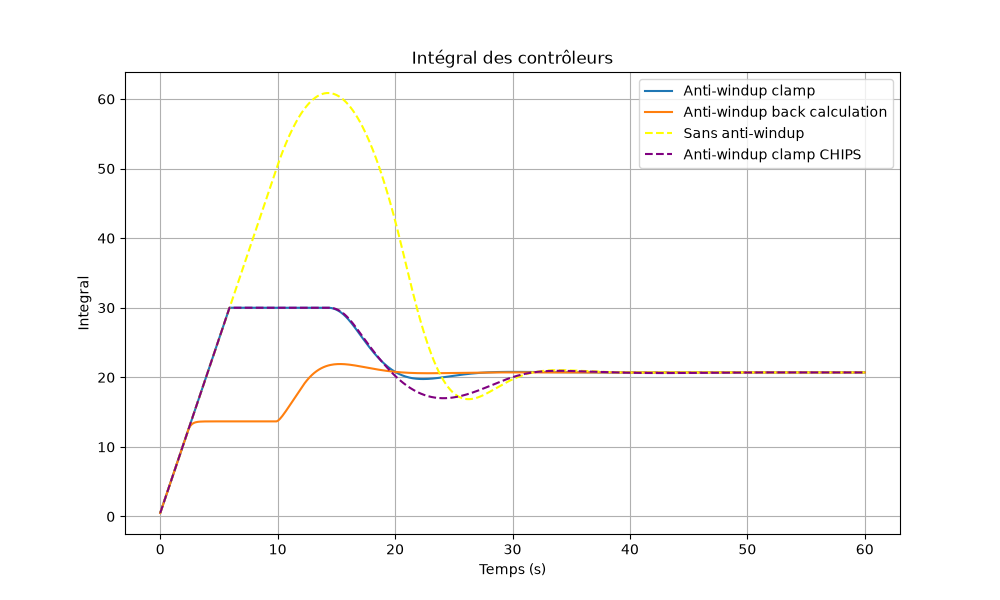
\includegraphics[width=\textwidth]{images/clamp_anti_windup_chips_integral.png}
    \caption{Les différentes intégrales des anti-windups comparées à l'anti-windup clamp en CHIPS}
    \label{clamp_anti_windup_chips_integral}
\end{figure}

\begin{figure}
    \centering
    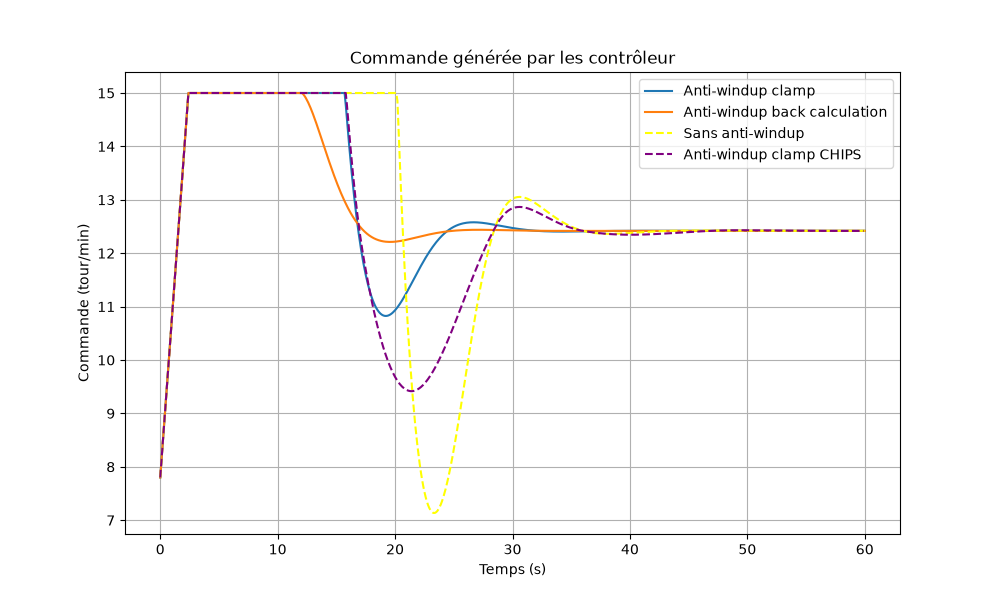
\includegraphics[width=\textwidth]{images/clamp_anti_windup_chips_blade.png}
    \caption{Les différentes vitesses de rotation des hélices avec différents anti-windups comparés à l'anti-windup clamp en CHIPS}
    \label{clamp_anti_windup_chips_blade}
\end{figure}

\begin{figure}
    \centering
    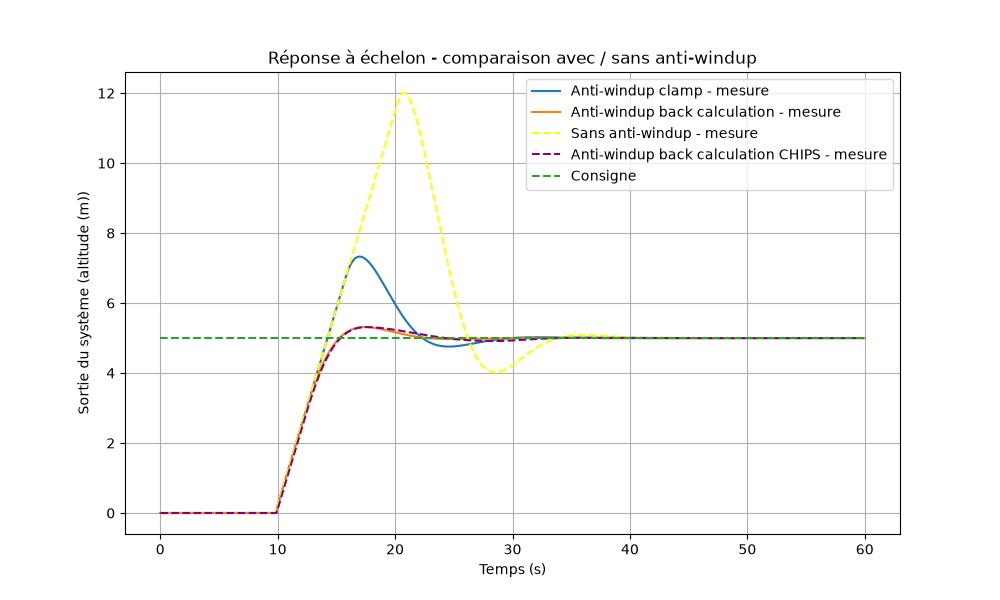
\includegraphics[width=\textwidth]{images/back_calculation_anti_windup_chips_altitude.png}
    \caption{Les différentes altitudes du drone avec différents anti-windups comparés à l'anti-windup back-calculation en CHIPS}
    \label{back_calculation_anti_windup_chips_altitude}
\end{figure}

\begin{figure}
    \centering
    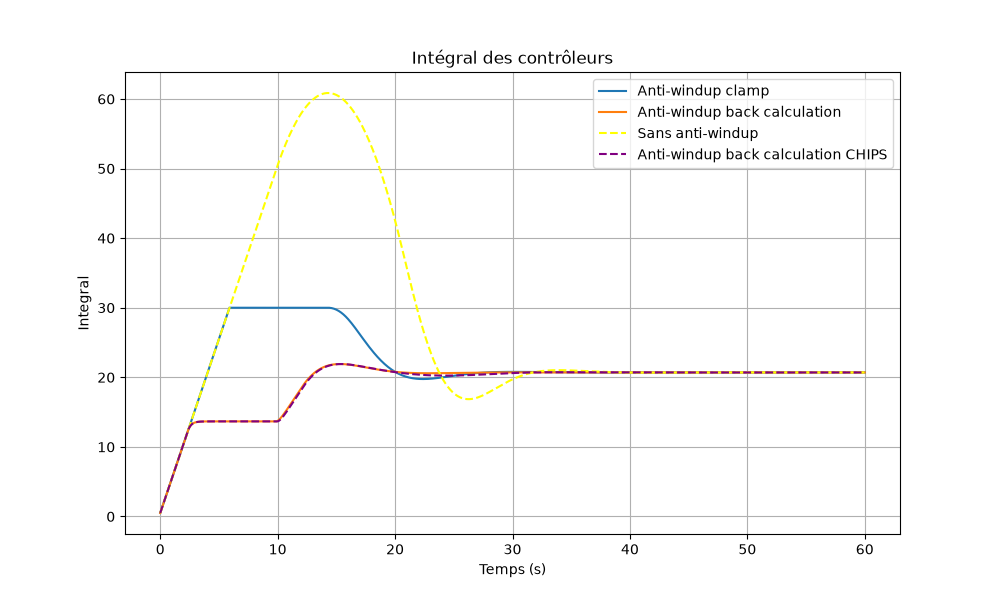
\includegraphics[width=\textwidth]{images/back_calculation_anti_windup_chips_integral.png}
    \caption{Les différentes intégrales des anti-windups comparées à l'anti-windup back-calculation en CHIPS}
    \label{back_calculation_anti_windup_chips_integral}
\end{figure}

\begin{figure}
    \centering
    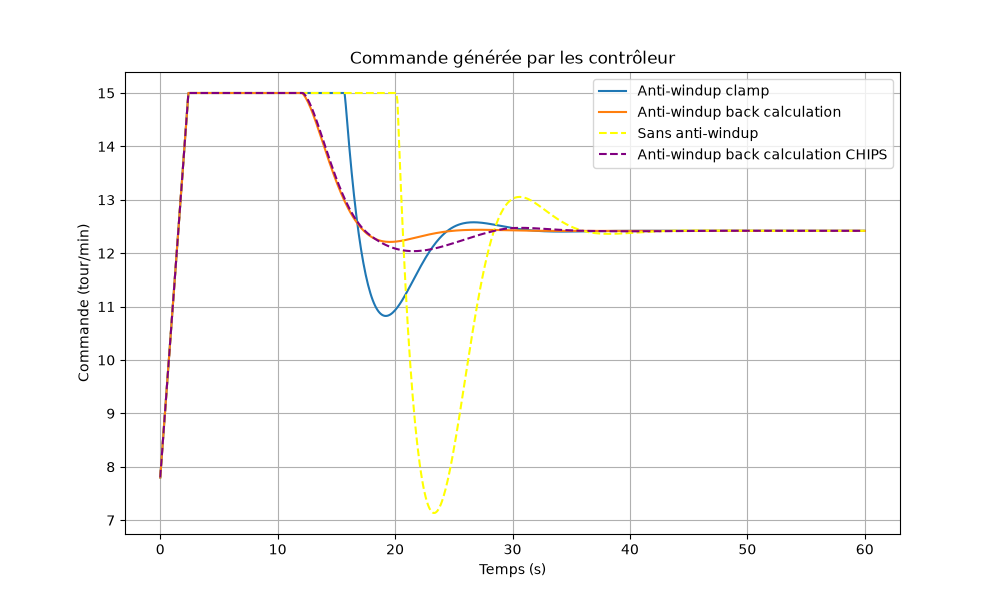
\includegraphics[width=\textwidth]{images/back_calculation_anti_windup_chips_blade.png}
    \caption{Les différentes vitesses de rotation des hélices avec différents anti-windups comparés à l'anti-windup back-calculation en CHIPS}
    \label{back_calculation_anti_windup_chips_blade}
\end{figure}

\subsubsection{Les métriques de la chaîne d'outils}
\label{metrique_toolchain}

Grâce à la chaîne d'outils, à partir d'un programme CHIPS qui fait 65 lignes, on obtient un programme BIP qui fait 600 lignes de code avec toute la logique interne des composants. Ce qui montre qu'un programme CHIPS est beaucoup plus compact qu'un programme BIP et qu'il abstrait certains détails d'implémentation de BIP. \\

Étant donné que la plus grosse partie de la chaîne d'outils est la compilation des programmes C++ générés par le compilateur BIP, nous avons mesuré les différents temps d'exécution de la chaîne d'outils pour le programme CHIPS du drone. Pour la partie de l'interprétation du programme CHIPS à la génération du programme BIP, il faut 10.229702854 secondes, pour la génération du code C++ à partir du programme BIP ainsi que sa compilation il faut 227.576063377 secondes, ce qui fait un temps total de 237.805766231 secondes, ce qui correspond à 3 minutes et 57 secondes pour la chaîne d'outils complète. \\

Pour information, la chaîne d'outils a été exécutée sur un ordinateur avec les caractéristiques suivantes :
\begin{itemize}
    \item Système d'exploitation : Ubuntu 24.04.4 LTS
    \item Processeur : Intel(R) Core(TM) i5-8250U CPU @ 1.60GHz
    \item Mémoire vive : 16 GB DDR4
\end{itemize}

\FloatBarrier

\newpage